% !Tex root = ../main.tex

\chapter{在隐私保护方面的应用}\label{chp:application}

% 在这一章,我们主要调研了近年来发表在安全顶会上的论文,

这一章我们主要介绍布隆过滤器及其衍生数据结构在隐私保护相关协议中的应用。
其中涉及的协议包括对称可搜索加密、隐私信息检索和隐私集合运算。
% 其中
% 本章涉及到的协议包括可搜索加密、隐私信息检索和隐私集合运算。
% 我们挑选了近年来
% 我们挑选了近年来发表在顶会上的论文,通过
% 可搜索加密、隐私信息检索和隐私集合计算三个密码学协议,并结合近年来发表的工作

\section{在对称可搜索加密方面的应用}

\subsection{背景介绍}

% 可搜索加密的定义,分类,系统模型
% 可搜索加密(searchable encryption)针对的外包加密文件上的搜索问题。
随着近年来数据规模的不断增大,越来越多的个人和企业选择将本地文件外包到云平台(如 iCloud、Amazon S3)进行存储。
% 数字化程度不断提高,文件
存储在云端的文件不仅为用户节省了本地存储所需要的成本,规避文件丢失的风险,还能让用户随时随地通过互联网对文件进行搜索和访问,极大地提高了便利性。
但是将文件直接存放在云服务器中也大大增加文件泄露的风险。
% 对于服务器内部来说,云服务提供商可以直接获取存储的文件;而
一方面云服务提供者可以直接获取文件,另一方面由于云服务器处在公开的网络环境中,很容易受到外部攻击者的攻击。
一旦文件遭到泄露,用户的隐私也受到威胁。
保护用户文件隐私的直接方式是将文件在本地进行加密,再将加密后的文件进行上传。
但是服务器无法在加密后的文件上执行搜索,用户需要搜索时只能把所有文件下载下来才能完成,这就丧失了将文件存储在云端的意义。
% 上传之前对文件加密,
% 但是这样一来服务器便无法对数据进行搜索,丧失了

为了解决文件隐私和可搜索之间的矛盾,对称可搜索加密(Searchable Symmetric Encryption,SSE)~\cite{song2000practical,curtmola2006searchable}的概念被提出。
对称可搜索加密通过为加密数据构造安全索引实现隐私保护的关键词搜索。
如图~\ref{fig:sse_protocol}~所示,对称可搜索加密中包含用户和服务器两个实体。
\begin{figure}[ht]
  \centering
  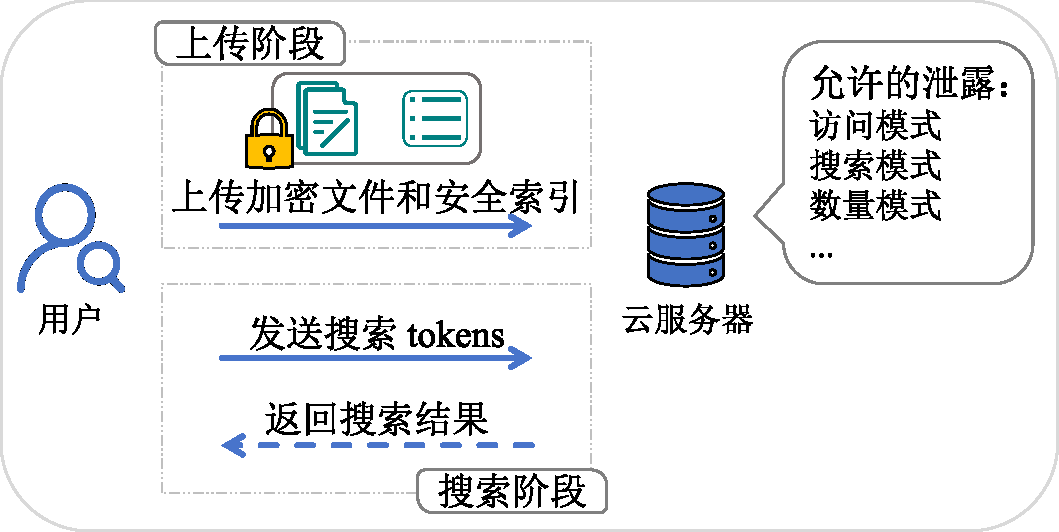
\includegraphics[width=0.8\textwidth]{figures/sse_pro.pdf}
  \caption{对称可搜索加密系统模型}
  \label{fig:sse_protocol}
\end{figure}
在上传阶段,用户不仅需要上传加密文件,还需要上传对应的安全索引。
在搜索阶段,用户根据需要搜索的关键词生成搜索 tokens,服务器使用搜索tokens检索得到加密的文件标识并返回给用户。

% 从对称可搜索加密的搜索过程可以看出,
我们假设服务器是半诚实的(semi-honest),即服务器会诚实地执行协议,但同时它会尝试通过分析输入输出信息来推断用户的隐私信息。
相比其他隐私保护的搜索方案,对称可搜索加密方案能在效率和安全之间取得更好的平衡。
% 在效率和安全之间
一方面,基于属性保留加密(Property-Preserving Encryption)的方案~\cite{bellare2007deterministica}虽然可以直接保留密文中的相等关系,从而实现高效的搜索。
但服务器可以通过分析密文上的相等信息来执行频率统计攻击并还原明文信息~\cite{naveed2015inferencea}。
在另一方面,基于通用密码学工具(如同态加密、安全多方计算以及不经意随机访问机)虽然能够提供较强的安全性,但这些工具要么在计算上开销非常大,要么存在较大的通信开销,直接应用到加密搜索场景会面临效率问题~\cite{ren2023searchable}。
% 同态加密或多方安全计算虽然能够提供较强的安全性,但同态加密方案需要
而对称可搜索加密通过将搜索过程转移到安全索引上,在允许有限信息泄露的同时提供了高效的搜索。

目前安全索引大多以倒排索引形式构建,也就是使用关键词信息去匹配文件标识的形式。
这样能够保证搜索效率只与关键词对应的文件数有关,而与整个数据库的大小无关。
对称可搜索加密允许泄露的信息也被称作模式信息(pattern information),这些信息包括:
\begin{itemize}
  \item 搜索模式(search pattern),即两次搜索是否包含相同的搜索关键词。
  \item 访问模式(access pattern),即每次搜索能匹配到哪些加密结果。
  \item 数量模式(volume pattern),即每次搜索返回的结果数量。
\end{itemize}
% 允许泄露这些信息是为了
对称可搜索加密协议的安全性是定义在给定的模式信息之上的,也就是说如果我们声称一个对称可搜索加密协议是安全的,那么除了允许泄露的模式信息之外,它不会泄露其他的任何信息。
% 所以说对称可搜索加密方案是牺牲一定的安全性来换取搜索效率。
近些年有大量工作~\cite{cash2015leakageabuse,grubbs2018pump,gui2019encrypted,blackstone2020revisiting,ning2021leap,kamara2022sok}集中关注于如何利用这些模式信息来设计相应的攻击,这些攻击被统称为泄露滥用攻击(Leakage-Abuse Attacks, LAAs)。
而我们前面的介绍的过滤器及其衍生数据结构正好可以用来隐藏特定的模式信息,从而避免受到对应的攻击。
以下我们将给出两个具体例子,介绍这些数据结构是如何用到对称可搜索加密之中的。

% 索引形式,倒排索引

\subsection{HXT}

这一节我们介绍的是 HXT (Hidden Cross-Tags) 协议~\cite{lai2018result}。
HXT 是一个针对连接多关键词查询的可搜索加密协议。
上一节介绍的背景都是默认只考虑单关键词查询,如果要扩展到多关键词并不是一件容易的事。
最直接的方式是执行多次单关键词的查询,但这样做,一来服务器与用户之间交互次数太多,通信开销太大;二来服务器可以知道每次查询的各种模式信息。
针对这些问题,Cash等人~\cite{cash2013highlyscalable}提出了次线性(sublinear)的连接多关键词协议 OXT (Oblivious Cross-Tags),即对于任意形如 $w_1\land w_2 \land \dots \land w_n$ 的连接多关键词查询,OXT 的查询复杂度只与第一个关键词对应的文件数量有关(即次线性),与查询的关键词数量、数据库中文件数量无关。
OXT 协议中包含两个索引,分别为 T-set 和 X-set,其中 T-set 与倒排索引类似,X-set 则是存储每个关键词 $w$ 与文件标识 $ind$ 配对的加密形式(称为 xtag)。
% 元组,如 $(w, ind)$ 形式。
% 通过构造两个索引
搜索时,用户首先选取搜索关键词中对应预估文件数最低的关键词(称为 s-term)生成对应在 T-set 中的搜索token(称为 stag),并生成其他搜索关键词(称为 x-term)对应的搜索tokens(称为 xtokens)。
以形如 $w_1 \land w_2 \land \dots \land w_n$ 的连接多关键词为例,其中假设 s-term 为 $w_1$。
服务器在收到这些搜索tokens之后,首先根据 stag 从 T-set 中检索出 $w_1$ 对应的加密文件标识列表和盲化的关键词与文件标识配对列表。
然后在上一步检索结果的基础上,使用 xtokens 还原出对应的 xtag,如果该 xtag 存在于 X-set 中,则返回对应的加密文件标识。
% 再利用 xotkens
% 与这些盲化的关键词与文件标识配对
图~\ref{fig:oxt_example}~对OXT协议的搜索过程进行了描述。
从整体上来看,OXT 协议的核心思路是先通过 T-set 确定出一个较小的文件范围,再使用 X-set 从这些文件中筛选出符合条件的结果。
这样就避免了前面提到的交互次数太多和泄露每个单独关键词模式信息的问题,而且能够实现次线性的搜索复杂度。
% 就能将搜索复杂度限制为 s-term 对应的文件数量。
但是在 OXT 协议中,因为需要计算出每个 x-term 与 s-term 对应的文件标识配对的 xtag,而服务器可以判断每一个 xtag 是否存在于 XSet 中。
以图~\ref{fig:oxt_example}~中的查询为例,服务器可以判断出关键词 $w_2$ 与 $ind_1$ 配对的 xtag 存在于 X-set,而关键词 $w_3$ 与 $ind_1$ 配对的 xtag 不存在于 X-set。
Lai 等人~\cite{lai2018result} 将这种信息定义为关键词对结果模式 (Keyword Pair Result Pattern, KPRP)。
而 HXT 协议的提出就是为了解决 OXT 中 KPRP 信息泄露问题。
% 为了防止 KPRP 的信息泄露,
% OXT 协议的
\begin{figure}[ht]
  \centering
  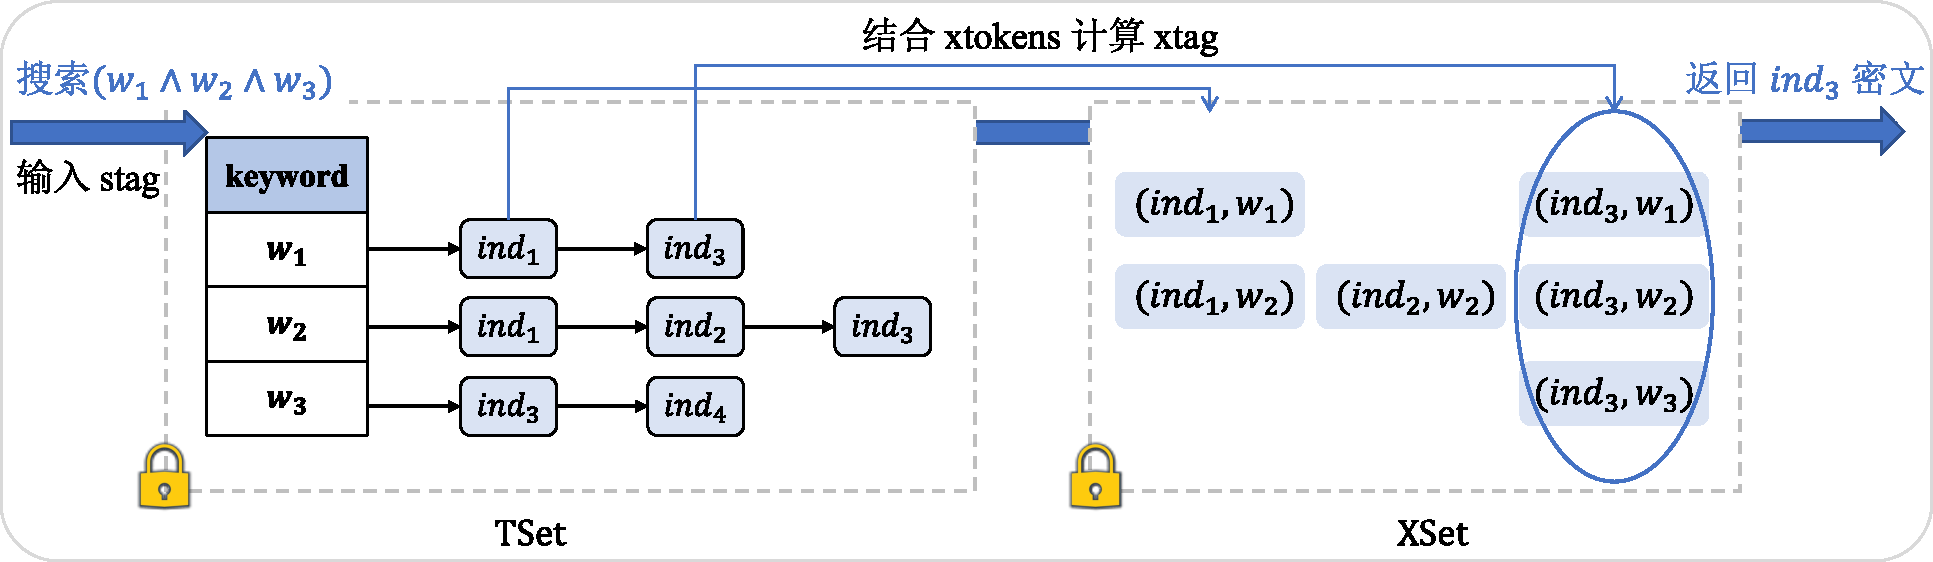
\includegraphics[width=\textwidth]{figures/OXT_exp.pdf}
  \caption{OXT 协议查询流程示例}
  \label{fig:oxt_example}
\end{figure}

HXT 协议相比 OXT 协议主要修改的是 X-set 构造。
为了隐藏 KPRP,就需要保证服务器不能通过计算 xtag 来完成在 X-set 中的筛选,也就是说 X-set 中不能直接保存 xtag。
% 因此在 HXT 协议中,
HXT 协议采用的方法是将 X-set 使用布隆过滤器构造成长度为 $m$ 的数组,再通过对称隐藏向量加密 (Symmetric Hidden Vector Encryption, SHVE) 进行加密,将加密结果作为 HXT 中的 X-set,转换过程如图~\ref{fig:xset_example}~所示。
\begin{figure}[ht]
  \centering
  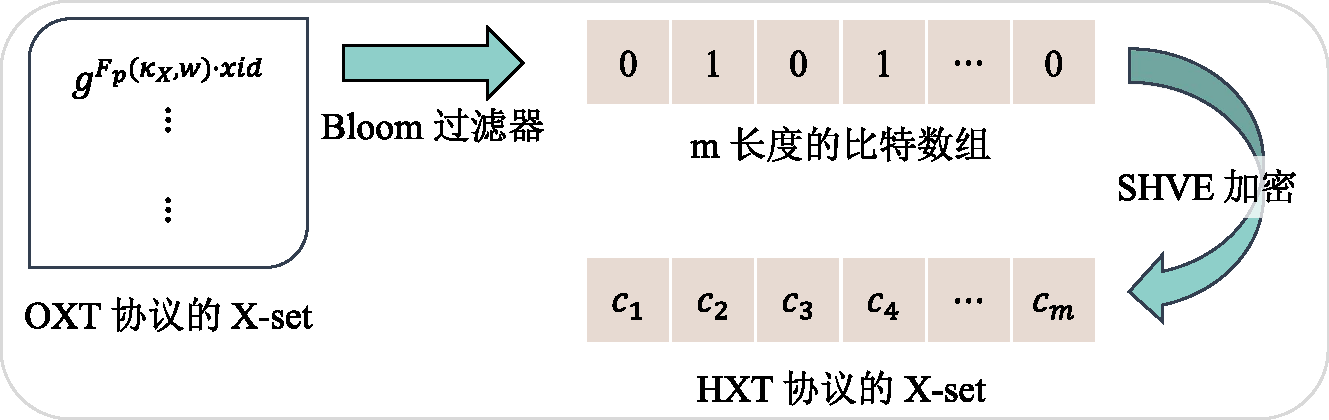
\includegraphics[width=0.95\textwidth]{figures/xset_exp.pdf}
  \caption{HXT 协议中 X-set 的构造}
  \label{fig:xset_example}
\end{figure}

其中,SHVE 是一种针对 $0/1$ 比特向量的加密算法,主要包含以下四个算法:
% 特点是当查询向量能够与加密的向量成功匹配时,SHVE
\begin{itemize}
  \item $\mathsf{SHVE}.\mathsf{Setup}(\lambda) \to msk$:通过输入安全参数 $\lambda$,输出主密钥 $msk$,并定义明文空间 $\mathcal{M}$。
  \item $\mathsf{SHVE}.\mathsf{KeyGen}(msk, \mathbf{v} \in \{0,1,*\}^m \to \mathbf{s} $:通过输入长度为 $m$ 的预测向量 $\mathbf{v}$ 和主密钥,输出解密密钥 $\mathbf{s}$。
  \item $\mathsf{SHVE}.\mathsf{Enc}(msk, \mu\in \mathcal{M}, \mathbf{x} \in \{0,1\}^m ) \to \mathbf{c}$:通过输入明文消息 $\mu$ 和长度为 $m$ 的索引向量 $\mathbf{x}$,输出密文 $\mathbf{c}$。
  \item $\mathsf{SHVE}.\mathsf{Query}(\mathbf{s}, \mathbf{c}) \to \mu \mbox{ or} \perp$:通过输入预测向量 $\mathbf{v}$ 对应的解密密钥 $\mathbf{s}$ 和密文 $\mathbf{c}$,如果$P_{\mathbf{v}}^{\mathsf{SHVE}}(\mathbf{x}) = 1$,则返回明文消息 $\mu$;否则返回 $\perp$。
\end{itemize}
其中 $P_{\mathbf{v}}^{\mathsf{SHVE}}(\mathbf{x})=1$ 的含义是向量 $\mathbf{v}$ 和 $\mathbf{x}$ 除了通配符 $*$ 所在位置上,其他所有位置上的值都相等,即
\begin{equation}
  P_{\mathbf{v}}^{\mathsf{SHVE}}(\mathbf{x}) = \left\{
  \begin{array}{ll}
  1 & \forall 1\leq i \leq m \  (v_i = x_i \mbox{ or } v_i=*), \\
  0 & \mbox{otherwise}. \\
  \end{array}
  \right.
\end{equation}
关于方案的具体构造可以参考文献~\cite{lai2018result},这里就不详细介绍。
% 这里我们不介绍
这里主要介绍 HXT 是如何结合 SHVE 来隐藏 KPRP 的。
构造时,用户使用图~\ref{fig:xset_example}~中的方式构造 X-set,在使用 SHVE 加密时,明文消息 $\mu$ 设置为 True。
% 在生成 stag 和 xtoken 部分,HXT 与 OXT 类似。
搜索时,用户还是首先生成 stag 和 xtoken,这部分 HXT 与 OXT 相同。
服务器还是通过 stag 检索 T-set,再利用 xtoken 计算出一系列 xtag。
% 在服务器收到
由于此时 X-set 中并没有直接存储 xtag,所以服务器并不能直接通过 xtag 完成判断。
% 与布隆过滤器的
对于服务器使用 stag 检索出的每个加密文件标识,后续的判断过程如下:
\begin{itemize}
  \item 服务器使用布隆过滤器的哈希函数,计算 xtag 对应的位置,并返回给用户。
  \item 用户生成长度为 $m$ 且所有位置为 $*$ 的向量 $\mathbf{v}$,根据服务器返回的位置,将向量 $\mathbf{v}$ 上所有这些位置上的值设为 $1$。
  \item 用户调用 $\mathsf{SHVE}.\mathsf{KeyGen}$ 将生成向量 $\mathbf{v}$ 对应的解密密钥 $\mathbf{s}$ 并发送给服务器。
  \item 服务器调用 $\mathsf{SHVE}.\mathsf{Query}$ 来判断 $\mathbf{v}$ 是否能与 X-set 匹配,如果返回为 True,则将对应的加密文件标识返回给用户。
\end{itemize}
相比于 OXT 协议,HXT 在搜索时需要多一轮通信,目的是让用户生成判断向量 $\mathbf{v}$。
%
% 从上述搜索过程可以看出,
得益于布隆过滤器的特性,向量 $\mathbf{v}$ 记录了所有 x-term 的信息,服务器只能判断每个加密文件标识是否满足查询条件中的 x-term,并不能判断每个单独的 x-term 与加密文件标识的对应关系,从而避免 KPRP 信息的泄露。
% 服务器只能判断每个加密文件标识是否满足查询条件,从而避免
% 对于服务器而言,

% 在 HXT 协议中,X-set 不再存储
% HXT~\cite{lai2018result}
% 本节我们介绍的协议

\subsection{XorMM}

这一节介绍的 XorMM~\cite{wang2022practical}是一个借助异或过滤器隐藏数量模式的对称可搜索加密协议。
数量模式指的是在搜索过程中,服务器获取的查询结果数量信息。
% 在早期的可搜索加密中,
早期的可搜索加密方案中认为这类模式信息的泄露是可以接受的。
但近年来的研究~\cite{grubbs2018pump,gui2019encrypted,blackstone2020revisiting}指出,攻击者可以利用数量模式推测用户搜索的关键词甚至还原出用户存储的信息。
因此隐藏数量模式就显得尤为重要。

要隐藏数量模式,最直接的思路是采用填充的方式,也就是将倒排索引中每个关键词对应的文件数量填充为相同的长度。
% 每次搜索强制让服务器返回相同数量的结果。
% 因此服务器就需要存储
这样无论是搜索哪个关键词,服务器查找得到的结果数量都相同,从而隐藏了每个关键词实际对应的数量模式信息。
现有工作~\cite{ando2022cost}认为,要实现隐藏数量模式信息的目的,填充后每个关键词对应的结果数量至少为填充前结果数量的最大值。
% 但是直接填充的话
这也就意味着填充后索引的存储开销会非常大,在实际中不可行。

为了解决这一问题,XorMM~\cite{wang2022practical}提出将异或过滤器的结构作为可搜索加密中的索引。
% 我们暂时不考虑对关键词和文件标识的加密,
以关键词 $w_1$ 对应文件标识 $\{ind_1, ind_2, ind_3\}$ 为例,XorMM 中将其看作 $\{(w_1 ||1, ind_1), (w_1 || 2, ind_2), (w_1 || 3, ind_3)\}$ 这样的键值型组合集合。
这样一来便可以使用异或过滤器对其进行记录,比如将 $ind_1$ 看作 $w_1 || 1$ 对应的指纹,查询时只需要输入 $w_1 || 1$,则返回对应的 $ind_1$。
而对于不存在的键,比如 $w_1||4$,还是能够得到其对应的结果。
% 为了确保
以上描述的是明文索引的构造思路,对于安全索引,我们只需要将所有的关键词替换成对应的关键词 token,而文件标识也需要替换成对应的密文形式。
这样构造的安全索引就能在不需要填充的情况下实现对任意查询都能返回一个确定的结果。
% 在构造索引之前,需要将

% 尽管采用异或过滤器
按照上述方式构造的安全索引能够实现较低的存储开销,但用户在查询时还存在通信开销上的问题。
假设 $\ell$ 为数量模式的最大值,为了隐藏数量模式,就需要每次搜索时让服务器都返回 $\ell$ 个搜索结果。
以查询关键词 $w_1$ 为例,用户需要发送 $\{w_1 || 1, w_1 ||2, \dots, w_1 || \ell \}$ 对应的搜索 tokens,这会造成非常大的通信开销。
为了解决这个问题,XorMM 采用受限伪随机函数(Constrained Pseudorandom Function, CPRF)让服务器可以根据用户给定的密钥独自生成 $\ell$ 个搜索 tokens,从而避免通信开销问题。
图~\ref{fig:xormm_example}~给出了XorMM协议的查询流程,描述如下:
% 主要分为以下几个步骤:
\begin{itemize}
  \item 用户根据查询关键词生成对应的 CPRF 密钥 $tk_{key}$,以及设定的返回结果数量 $\ell$,并发送给服务器。
  \item 服务器根据 $tk_{key}$ 生成 $\ell$ 查询关键词对应的 $\ell$ 个搜索 tokens,并通过异或过滤器得到 $\ell$ 个对应的结果,最后将结果返回给用户。
\end{itemize}
\begin{figure}[ht]
  \centering
  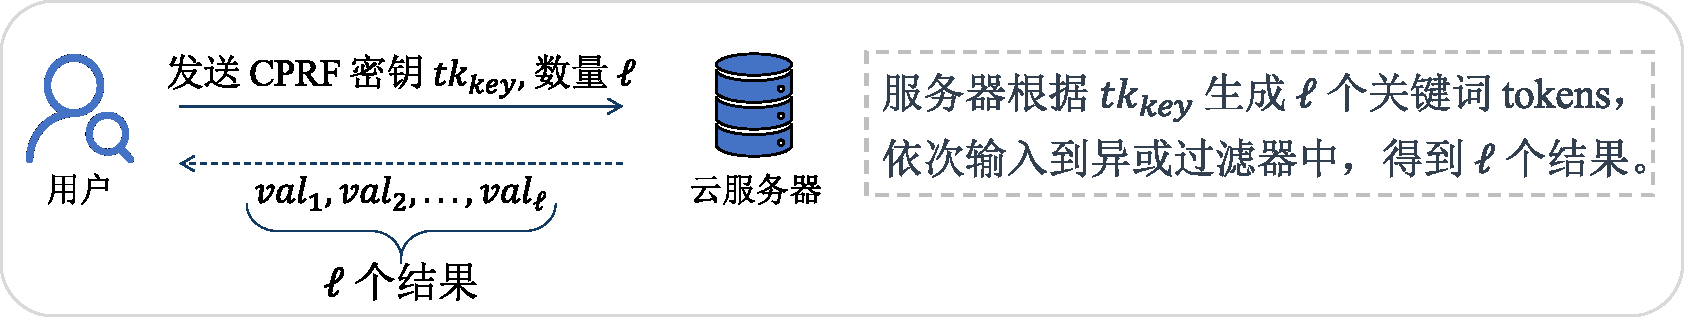
\includegraphics[width=\textwidth]{figures/xormm_exp.pdf}
  \caption{XorMM 协议查询示例}
  \label{fig:xormm_example}
\end{figure}

在XorMM的协议设计中,我们可以发现异或过滤器的作用更像是不经意键值存储,也就是说返回的结果是查询键对应的值,而不是简单的判断。
% 正如我们在
因为对于任意查询输入,不经意键值存储都会返回一个确定的值。
所以在XorMM协议中,对于任意查询都返回 $\ell$ 个对应的结果,这就实现了在不需要填充的情况下,隐藏数量模式的信息。

既然XorMM协议中将异或过滤器看作不经意键值存储来使用,那么很自然可以想到使用其他的不经意键值存储来代替XorMM协议中的异或过滤器。
% 最近的工作~\cite{}
Bienstock等人~\cite{bienstock2023NearOptimal}将XorMM中的异或过滤器替换为 RB-OKVS 设计了 RB-MM 协议,从而将存储开销从 $1.23n$ 降低为 $1.03n$。

\section{在隐私信息检索方面的应用}

\subsection{背景介绍}

隐私信息检索 (Private Information Retrieval, PIR) 是一种用于隐藏用户查询内容的隐私保护密码协议。
如图~\ref{fig:pir_protocol}~所示,隐私信息检索协议中存在用户和服务器两个实体。
\begin{figure}[ht]
  \centering
  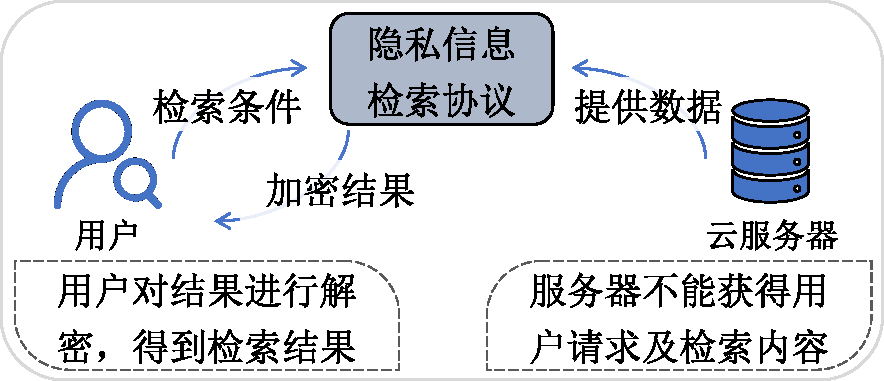
\includegraphics[width=0.72\textwidth]{figures/pir_pro.pdf}
  \caption{隐私信息检索系统模型}
  \label{fig:pir_protocol}
\end{figure}
对于用户只需要输入检索条件,并能得到相应的检索结果。
而检索的数据则由服务器提供。
与可搜索加密相比,隐私信息检索针对的场景和考虑的问题都有所区别。
在场景上,可搜索加密针对的是外包数据存储场景,也就是云服务器中存储的是用户的数据,典型的是各种云盘服务;而隐私信息检索中所有的数据是由服务器自身掌握的,也就是数据本身并不是属于查询用户的,比如像查询火车票服务。
由于数据的持有方不同,二者考虑的问题也就相差甚远。
在可搜索加密中,因为数据都是以加密形式存储在服务器,所以服务器能够获取到的信息是非常有限,此时只需要考虑服务器不能根据查询时泄露的各种模式信息推断出用户的查询内容或存储内容;在隐私信息检索中,因为服务器是直接掌握所存储的数据,所以可以直接根据返回的结果来判断用户的查询信息。
如何保护用户的查询隐私成为隐私信息检索的主要目标。

% 实现 PIR 的技术路线
根据实现方式,可以将隐私信息检索分为基于单服务器和基于双服务器两种方式。
在基于单服务器的方案中,用户与服务器的通信开销与存储条目数量成正比。
而服务器的计算开销也非常大,因为服务器必须要访问每一个存储条目,否则就会泄露当前用户没有查询到哪些内容的信息~\cite{beimel2004reducing}。
而基于双服务器的方案虽然相比单服务器的方案在计算开销上要更低,但是这类方案需要假设两个服务器是不共谋的,这种安全假设太强,难以在现实中部署。
% 采用多方安全计算作为底层协议,

根据查询方式,隐私信息检索又分为基于索引 (index-based PIR) 和基于关键词 (keyword-based PIR) 两种类型。
顾名思义,在基于索引的隐私信息检索协议中,每条数据都对应一个索引 $i\in \{1, 2, \dots, n\}$,查询时用户通过索引得到需要查询的条目,而服务器并不能推断用户发送的索引信息;而在基于关键词的隐私信息检索协议中,每条数据对应一个关键词,查询时用户通过关键词得到需要查询的条目,服务器不能推断用户发送的关键词信息。
% 早期的工作大多围绕着基于索引的协议进行设计,近些年开始
% 设计一个隐私信息检索协议,往往需要结合多种密码协议,比如

% 安全假设,系统模型
本文介绍的是基于关键词的单服务器隐私信息检索方案。
我们假设服务器是半诚实的,即服务器会诚实地执行协议,但同时也会通过协议执行时获取的信息来推测用户的查询信息。
早期的基于关键词的隐私信息检索协议是通过执行对数轮基于索引的隐私信息检索协议来实现的。
近年来有一部分工作是借助全同态加密实现基于关键词的检索。
但相比于基于索引的协议,目前大部分基于关键词的协议无论在通信上还是在计算上依然存在开销较高的问题。
% 很高。
% 最近的工作~\cite{celi2024call}通过结合将同态加密与二进制引信过滤器进行结合,构建了高效的基于关键词的隐私信息检索方案。
% OT,HE

\subsection{ChalametPIR}

ChalametPIR~\cite{celi2024call}是由 Celi 和 Davidson 结合同态加密和二进制引信过滤器提出的一种计算高效且通信开销低的隐私信息检索方案。
% 最近 Celi 和 Davidson~\cite{celi2024call} 通过结合
从计算效率来看,ChalametPIR 相比现有基于关键词的隐私信息检索方案要快 $6$ 到 $11$ 倍。
% 相比现有基于关键词的隐私信息检索方案,ChalametPIR 的计算效率
在介绍 ChalametPIR 之前,我们首先介绍构造该协议需要用到的 Regev 同态加密方案~\cite{regev2009lattices}。

Regev 加密~\cite{regev2009lattices}是一种基于 LWE (Learning with Errors) 困难问题的加密方案,它可以支持同态加法操作。
简单来说,令 $p, q, n, \sigma$ 为 Regev 加密机制 $\Sigma_{\mathsf{lwe}}$的参数,$\lambda$ 为安全参数,它主要包含以下四个算法:
\begin{itemize}
  \item $\Sigma_{\mathsf{lwe}}.\mathsf{KeyGen}(1^\lambda, q, p, n, \sigma) \to (pp, sk)$:通过输入预先设定的参数,生成公共参数 $pp$ 和私钥 $sk$。
  % 随机生成私钥向量 $\mathbf{s}\gets \Chi_\sigma^n$,返回公共参数 $pp = (q, n, p, \Chi_\sigma)$ 和私钥 $sk = \mathbf{s}$。
  \item $\Sigma_{\mathsf{lwe}}.\mathsf{Enc}(pp, sk, \mathbf{v}\in \mathbb{Z}_p) \to c$:根据公共参数和私钥,对输入明文 $v$ 进行加密,输出密文结果 $c$。
  % 生成随机向量 $\mathbf{a} \gets \mathbb{Z}_q^n$ 和噪声向量 $e\gets \Chi_\sigma$,计算 $\hat{c} = sk \cdot $
  \item $\Sigma_{\mathsf{lwe}}.\mathsf{Eval}(pp, \mathbf{c} \in \mathbb{Z}_b^m, \mathbf{w} \in \mathbb{Z}_p^m)\to c'$:给定一组由相同密钥生成的密文 $\mathbf{c} = (c_1, c_2, \dots, c_m)$,以及明文向量 $\mathbf{w}$,输出密文 $c'$。
  \item $\Sigma_{\mathsf{lwe}}.\mathsf{Dec}(pp, sk, c) \to v$:给定公共参数 $pp$,私钥 $sk$,以及密文 $c$,输出对应的明文 $v$。
\end{itemize}
% 这里我们不展开介绍 Regev 加密机制的具体构造,

相比一般形式的加密,Regev 加密机制中多了一个 $\Sigma_{\mathsf{lwe}}.\mathsf{Eval}$ 算法。
其返回得到的密文 $c'$ 在解密后得到的是向量 $\mathbf{c}$ 对应的明文 $\mathbf{v}$  与向量 $\mathbf{w}$ 的内积。
这是由于 Regev 加密机制满足加法同态的性质而得到的。
关于 Regev 加密机制的具体构造这里就不展开介绍,感兴趣的可以参看文献~\cite{regev2009lattices}。

我们重点来说明 Regev 加密机制是如何用来构造隐私信息检索协议的。
近年来有一系列工作~\cite{davidson2023frodopir,henzinger2023one,zhou2023optimal}都是采用这种技术路线,这类协议也被称作 LWE-based PIR,下面就简记为 $\mathsf{LWEPIR}$。
% 我们将这类协议记为 LWE-based PIR。
% 采用这种技术路线设计的隐私信息检索协议也被称为 LWE-based PIR,~\cite{davidson2023frodopir,henzinger2023one,zhou2023optimal}
% 使用 Regev 加密机制构造
% 这类协议也称
$\mathsf{LWEPIR}$ 分为离线和在线两个阶段。
在离线阶段,服务器需要执行生成全局公共状态信息 (global public state),并将该信息共享给用户。
注意这里的离线阶段只需要执行一次。
在线阶段可以分为三个部分,首先由用户发起请求,然后服务器回应请求,最后用户将服务器返回的结果进行解密。
$\mathsf{LWEPIR}$ 的构造思路是将服务器上的数据看作 $m_1 \times m_2$ 的矩阵,即一共有 $m_1$ 行数据,每条数据长度为 $m_2$。
在离线阶段,服务器预先生成 $\Sigma_{\mathsf{lwe}}.\mathsf{Enc}$ 过程中用到的参数 $A$。
在查询过程中,以请求第 $i$ 行数据为例(假设我们这里考虑的是基于索引的协议),用户只需要生成长度为 $m_1$ 的全零查询向量,其中第 $i$ 个位置设为 $1$。
用户再随机生成私钥,调用 $\Sigma_{\mathsf{lwe}}.\mathsf{Enc}$并结合参数 $A$ 对查询向量进行加密,将加密结果发送给服务器。
服务器将本地 $m_1 \times m_2$ 的明文矩阵看作 $m_2$ 个长度为 $m_1$ 的列向量组成,对于每个列向量,将其与用户发送的加密向量作为输入,调用 $\Sigma_{\mathsf{lwe}}.\mathsf{Eval}$ 计算得到加密结果。最后将所有的加密结果返回给用户。
% ,将计算结果返回给用户。
% 以用户发送的加密向量和本地 $m_1 \times m_2$ 明文矩阵的列向量作为输入,调用 $\Sigma_{\mathsf{lwe}}.\mathsf{Eval}$,将计算结果返回给用户。
用户将结果解密便可以得到第 $i$ 行数据的信息。

$\mathsf{LWEPIR}$ 的正确性很容易进行验证。
因为 $\Sigma_{\mathsf{lwe}}.\mathsf{Eval}$ 计算的结果是输入两个向量的内积。
在该协议中,输入的两个向量分别是用户发送的加密查询向量和服务器上存储数据的列向量。
由此可以推出,假设用户查询的第 $i$ 行,服务器会依次得到第 $i$ 行上所有列的加密数值(因为是内积运算,只有第 $i$ 行为 $1$)。
在这一过程中,只要用户每次查询都是随机生成加密密钥,那么用户发送的加密向量对于服务器来说就是随机的,服务器无法通过用户的查询获取查询模式相关的信息。
而在查询过程中,服务器存储的数据上每一比特都参与了运算,因此服务器也无法获取访问模式相关的信息。
也就是说这样的设计能够满足隐私信息检索协议的隐私保护需求。
% 并将这些加密数值返回给用户。

但是以上的构造只是针对基于索引的协议来进行设计的。
ChalametPIR 通过引入二进制引信过滤器,将上述构造改造成了基于关键词的协议。
% 要改造成基于关键词的协议,那就需要引入过滤器结构,也就是 ChalametPIR 的构造思路。
% 由于二进制引信过滤器中记录的是每个元素对应的指纹值,ChalametPIR
% 具体来说,ChalametPIR 将
在使用关键词作为查询条件的情况下,服务器上存储的数据就可以看作键值型数据形式,即关键词作为键,对应的数据条目作为值。
那么直接的思路就是可以将这种数据采用异或型过滤器来构造。
\begin{figure}[ht]
  \centering
  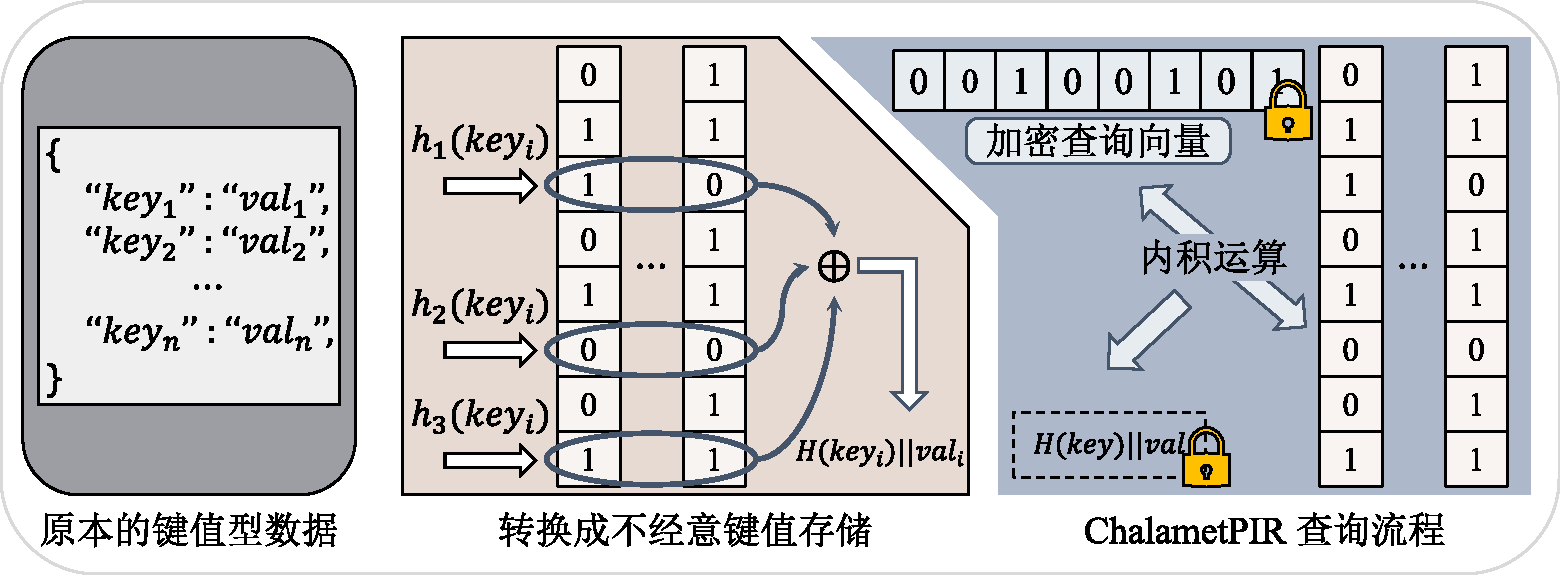
\includegraphics[width=\textwidth]{figures/pir_exp.pdf}
  \caption{ChalametPIR 协议构造思路}
  \label{fig:pir_exp}
\end{figure}
% 但是如果直接使用将元素看作关键词,元素的指纹值看作关键词对应的数据,那么服务器就会直接获取到用户的查询信息和查询结果。
ChalametPIR 协议的构造思路如图~\ref{fig:pir_exp}~所示,其中指纹函数被定义为 $f(key) = H(key) || val$,$H$ 为哈希函数。
这样在离线阶段,服务器需要额外生成过滤器的相关参数信息。
用户在查询时,与 $\mathsf{LWEPIR}$ 类似,也是先生成全零向量,再使用过滤器的哈希函数计算出所需要查询的关键词对应的位置,并在查询向量中将这些位置上的比特置为 $1$。
之后用户便采用相同的方法对向量进行加密,并把加密后的查询向量发送给服务器。
服务器调用 $\Sigma_{\mathsf{lwe}}.\mathsf{Eval}$ 以相同的方式对加密查询向量与本地构造的过滤器进行计算,将结果返回给用户。
用户将结果进行解密后便可以得到查询关键词对应的数据。
% ChalemetPIR 的构造利用了异或型过滤器本身具备的
由于异或型过滤器本身可以记录键值型数据,而且 $\mathsf{Evaluate}$ 的执行过程也可以看作内积操作,再得益于 Regev 加密算法对密文上求内积操作的支持,这些因素使得二者之间的组合可以实现基于关键词的隐私信息检索协议。

% 再通过使用参数 $A$
% 用户发起请求时,
% 也就是
% 对于服务器存储的数据,ChalametPIR 将其看作键值型数据结构,我们使用 $\{(key_1, val_1), (key_2, val_2), \dots, (key_n, val_n)\}$ 来表示。

\section{在隐私集合运算方面的应用}

\subsection{背景介绍}

隐私集合运算 (Private Set Operation, PSO) 是隐私保护计算领域中的一个重要分支,主要用于在不泄露集合数据的情况下,对两方或多个参与方各自私有集合执行安全运算。
% 安全地计算两个或多个参与方之间的集合
常见的隐私集合运算包括隐私集合求交 (Private Set Intersection, PSI) 和隐私集合求并 (Private Set Union, PSU) 两种。
% 在隐私集合求交协议中,
\begin{figure}[ht]
  \centering
  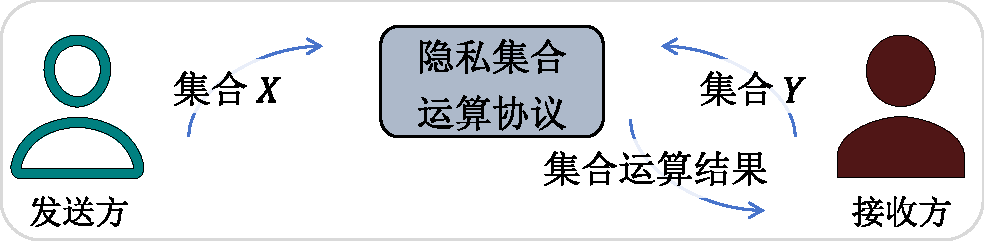
\includegraphics[width=0.72\textwidth]{figures/pso_pro.pdf}
  \caption{隐私集合运算系统模型}
  \label{fig:pso_protocol}
\end{figure}
本文中我们主要介绍两方参与的隐私集合运算协议,如图~\ref{fig:pso_protocol}~所示,这两个参与方分别是发送方和接收方。
在隐私集合求交协议中,发送方持有集合 $X$,接收方持有集合 $Y$。
协议执行完成后,发送方不会获得任何信息,接收方仅能获得 $X\cap Y$ 的信息。
同理,隐私集合求并协议要求接收方只能获得 $X\cup Y$ 的信息,而无法获得 $X\cap Y$ 的信息。
隐私集合运算在现实中有着广泛的应用前景~\cite{zhang2024survey},比如隐私集合求交可以用于联系人匹配、基因检测和模式匹配、传染病患者追踪等;隐私集合求并可以用于隐私保护数据聚合、合并IP黑名单进行网络风险评估等。

隐私集合运算协议常用的安全模型有半诚实模型和恶意模型。
在半诚实模型中,所有参与方都诚实地执行协议,但是也会尝试从其他参与方的输入或协议的中间计算结果中推断隐私信息。
在恶意模型中,参与方会主动去破坏协议的安全性,包括恶意篡改输入输出信息、拒绝参与协议、提前终止协议等。
在本文中,如无特殊说明,默认各参与方是半诚实的。
假设发送方和接收方分别持有集合 $X=\{x_1, x_2, \dots, x_{n_X}\}$ 和 $Y=\{y_1, y_2, \dots, y_{n_Y}\}$。
实现隐私集合运算协议的直接方式是让发送方和接收方对各自集合中的所有元素进行隐私保护的两两比较。
但当双方集合规模较大时,这样做会带来非常严重的通信和计算开销。
为了降低开销,隐私集合计算协议中通常需要引入各种特定的数据结构,如哈希表、过滤器和不经意键值存储~\cite{zhang2024survey}。

借助哈希表构造的协议流程如图所示。
\begin{figure}[ht]
  \centering
  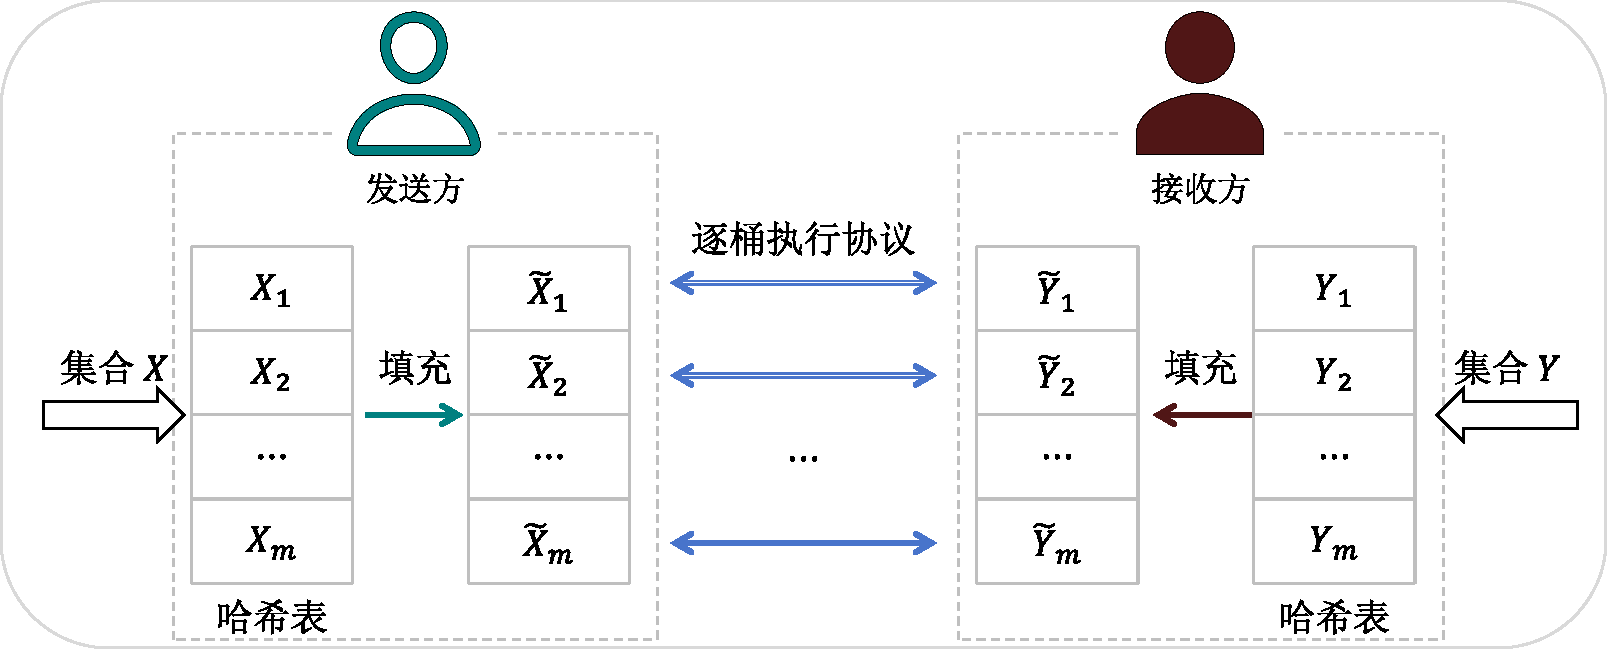
\includegraphics[width=\textwidth]{figures/pso_ht.pdf}
  \caption{基于哈希表构造的隐私集合运算协议流程}
  \label{fig:pso_ht}
\end{figure}
在该过程中,发送方和接收方利用哈希表将集合 $X$ 和 $Y$ 分别划分成 $m$ 个不相交的子集 $\{X_1, X_2, \dots, X_m\}$ 和 $\{Y_1, Y_2, \dots, Y_m\}$。
为了确保相同的元素能够映射到相同序号的子集中,双方需要使用相同的哈希函数进行构造。
这样双方就能通过哈希表完成集合元素的对齐。
之后双方在每个子集 $X_i$ 和 $Y_i$ 中填充一定数量的哑元得到 $\tilde{X}_i$ 和 $\tilde{Y}_i$。
最后双方在填充哑元后的 $\tilde{X}_i$ 和 $\tilde{Y}_i$ 上执行隐私集合计算协议。
这样做的好处是双方不再需要对所有元素进行两两比对,从而降低计算复杂度。
使用填充的目的是防止将桶中元素的数量暴露出来。
% 比如当发送方的集合 $X_i$ 为空,而接收方的集合 $Y_i$ 不为空时,接收方便可以判断出发送方没有 $Y_i$ 集合中对应的元素。
% 根据参与双方使用的哈希表结构可以将协议分成两类:
此类协议根据参与双方使用的哈希表结构不同主要可以分为两类:一类是双方都使用哈希表,再根据划分的每个子集中的元素构建多项式。
假设双方集合中的元素数量都为 $n$,构建的哈希表长度为 $m$,哈希表中每个桶的大小为 $b$,那么这种方法就把原本需要构造 $n$ 次多项式转换成构造 $m$ 个 $b$ 次多项式。
由于桶中容量最多为 $b=O(\log n)$,因此元素的比较次数从 $n^2$ 降低为 $O(n\log^2n)$。
% 从而降低计算复杂度。
另一类是一方使用布谷鸟哈希表,另一方使用一般形式的哈希表。
在前面我们也介绍过,布谷鸟哈希表中桶的大小为 $1$,而对于每个元素,它存放的位置可能是使用哈希函数映射后得到的位置中的一个。
在比较时,一方使用布谷鸟哈希表将元素 $x$ 存储在 $k$ 个哈希函数对应位置中的一个,另一方使用一般形式的哈希表将元素 $y$ 存储在 $k$ 个哈希位置上。
在逐个位置进行对比时,由于布谷鸟哈希中 $b=1$,此时比较次数进一步降低为 $O(n\log n)$。

% 借助过滤器构造的协议流程如图所示。
% 引入过滤器的目的是利用
基于过滤器构造的协议主要是利用过滤器的成员测试功能避免双方交互过程中直接发送原始数据集,从而防止出现通信开销过大的问题。
% 避免通信开销过大的问题。
% 过滤器的成员测试功能降低双方交互过程中的通信开销,
% 在隐私集合运算协议中引入过滤器的目的是降低通信开销
将过滤器应用到隐私集合运算主要有两种方式:一种是将数据集盲化后插入过滤器,其协议流程如图~\ref{fig:pso_ft1}~所示。
\begin{figure}[ht]
  \centering
  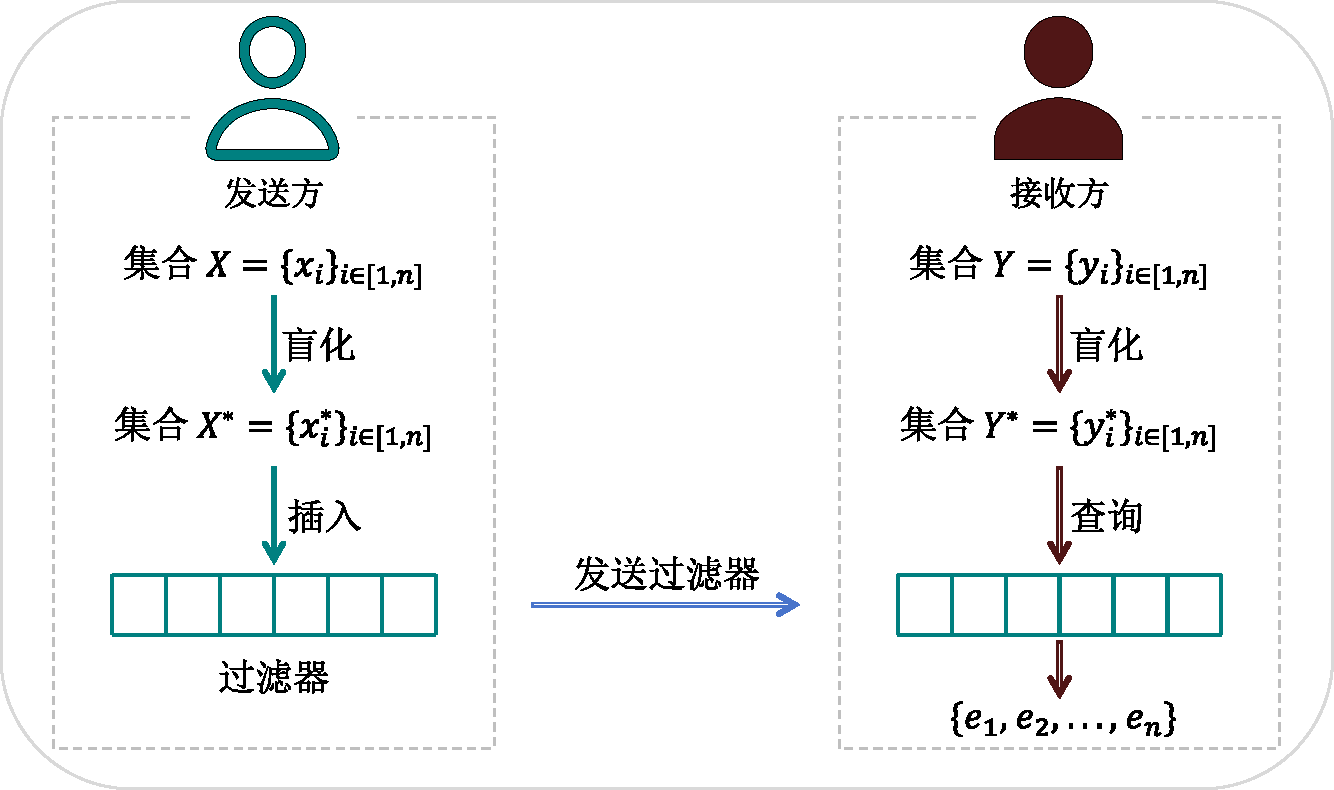
\includegraphics[width=0.9\textwidth]{figures/pso_ft1.pdf}
  \caption{基于过滤器和盲化技巧构造的隐私集合运算协议流程}
  \label{fig:pso_ft1}
\end{figure}
比如发送方将数据集 $\{x_i\}_{i\in[1,n]}$ 盲化后得到 $\{x^*_i\}_{i\in[1,n]}$ 并将盲化后的数据集插入过滤器。
由于盲化后的数据集并不会暴露原始集合,因此发送方直接将得到的过滤器发送给接收方。
接收方使用同样的方式对自己的集合进行盲化,并通过过滤器来判断哪些元素是与接收方相同的。
另一种是将数据集以明文的形式插入过滤器中并将过滤器加密,其协议流程如图~\ref{fig:pso_ft2}~所示。
\begin{figure}[ht]
  \centering
  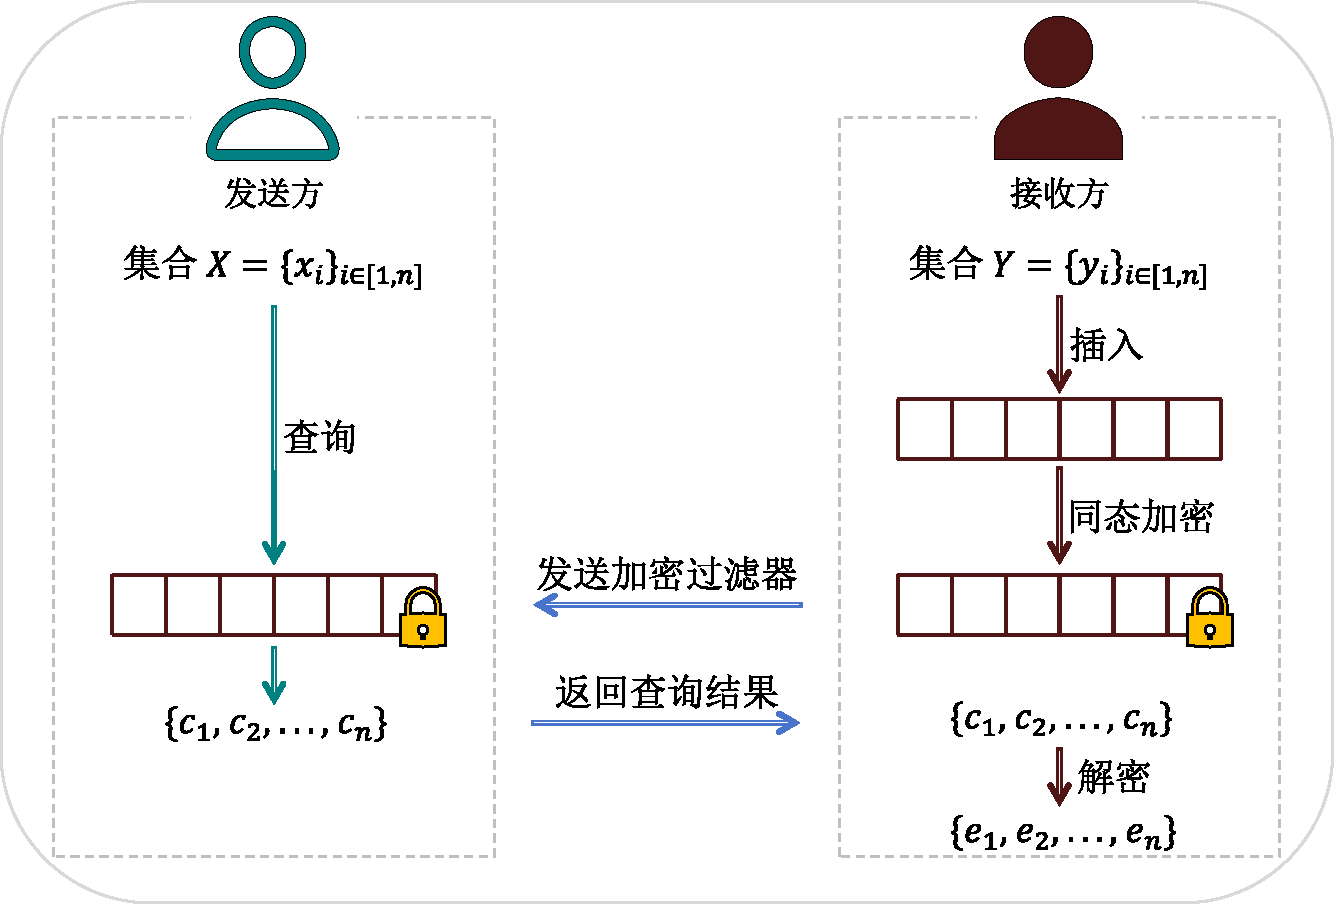
\includegraphics[width=0.9\textwidth]{figures/pso_ft2.pdf}
  \caption{基于过滤器和同态加密构造的隐私集合运算协议流程}
  \label{fig:pso_ft2}
\end{figure}
比如接收方将数据集 $\{x_i\}_{i\in [1,n]}$ 直接插入布隆过滤器中,再使用同态加密对布隆过滤器的每一个比特进行加密,并将加密结果发送给发送方。
发送方对自己集合中每个元素 $x_i$ 找到布隆过滤器上对应的位置,将对应位置上的密文进行相加,得到 $c_i$。
如果 $x_i\in Y$,那么 $c_i$ 应该是 $k$ 的密文(或者为 $0$ 的密文,取决于布隆过滤器是否逐比特反转),其中 $k$ 为布隆过滤器中哈希函数的数量。
发送方再将得到的密文发送给接收方,接收方解密后便可以判断出交集信息。
% 得到交集元素。
上述举得两个例子虽然都是计算交集,但也可以通过类似的方式改造成计算并集,这里就不详细介绍。
感兴趣的可以阅读文献~\cite{davidson2017efficient,chen2024private}。
% 使用这种方式
除了使用布隆过滤器之外,Resende 和 Aranha~\cite{resende2018faster} 提出了基于布谷鸟过滤器的隐私信息检索方案,与基于布隆过滤器构造的方案相比,该方案的通信开销更低。
% 能够提供更低的通信开销。
% 布谷鸟过滤器

近些年来有越来越多的工作是在不经意随机存储结构上构造隐私集合运算协议。
更准确地说,不经意键值存储结构本身就是从隐私计算求交协议~\cite{garimella2021oblivious}中总结出来的一种数据结构。
有许多隐私计算操作协议~\cite{kolesnikov2019scalable,garimella2021private,rindal2021volepsi,zhang2023linear}均显式或隐式地利用了不经意随机存储结构对集合数据进行编码。
此类协议主要利用了不经键值存储的不经意性,也就是对于映射关系 $x_i \mapsto v_i$,当 $v_i$ 为随机值时,不经意键值存储结构能够隐藏其对应的键 $x_i$。
对应到隐私集合运算协议中,$x_i$ 一般对应参与者集合中的元素,而 $v_i$ 一般对应协议中的关键辅助信息。
协议的执行流程如图所示。
\begin{figure}[ht]
  \centering
  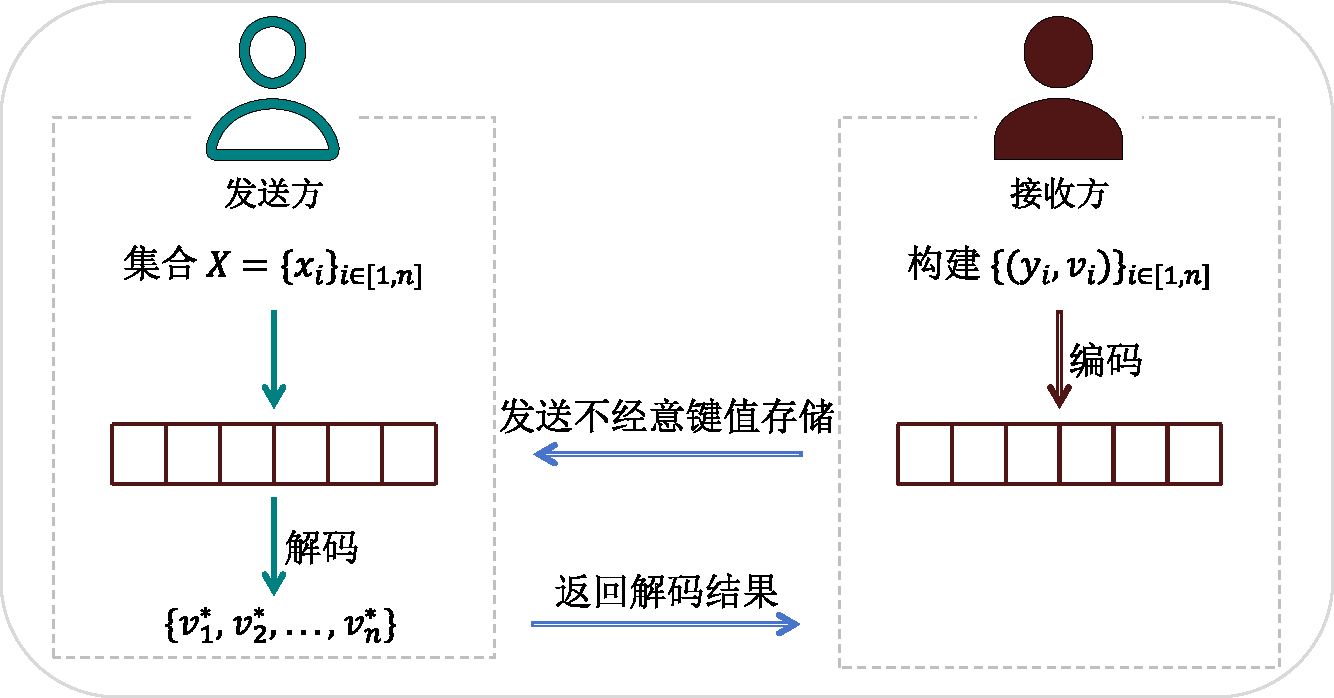
\includegraphics[width=0.9\textwidth]{figures/pso_okvs.pdf}
  \caption{基于不经意键值存储构造的隐私集合运算协议流程}
  \label{fig:pso_okvs}
\end{figure}
% 使用不经意随机存储结构构造的协议流程如图所示。
接收方随机生成与元素对应的关键辅助信息 $\{v_i\}_{i\in [1,n]}$,以此构建键值对数据 $\{(y_i, v_i)\}_{i\in [1,n]}$,并使用不经意随机存储编码,将编码后的结果发送给发送方。
发送方将自己的集合元素作为输入,在收到的编码结果进行解码,得到一系列的 $\{v^*\}_{i\in [1,n]}$。
最后双方可以根据集合 $\{v_i\}_{i\in [1,n]}$ 和 $\{v_i^*\}_{i\in [1,n]}$ 的信息进一步来完成求交集或并集的操作。
另外,不经意键值存储也可以用于前面基于哈希表的构造中来提高安全性。
在基于哈希表构建的隐私集合求交协议中,如果是在恶意安全模型假设下,恶意参与者可以选择将交集元素存放在其映射位置上的其中一个而非所有位置,这样就会对协议造成破坏。
而如果使用不经意键值存储,因为所有的存储对象是以异或拆成多份存储的,避免上述问题的出现。
接下来我们着重介绍两个基于不经意键值存储构造的隐私集合求交协议 VOLE-PSI~\cite{rindal2021volepsi}和隐私集合求并协议 SKE-PSU~\cite{zhang2023linear}。

% 利用键值对 $\{x_i ,v_i\}_{i\in [n]}$ 构造不经意
% \subsection{方案介绍}

\subsection{VOLE-PSI}

VOLE-PSI~\cite{rindal2021volepsi}是结合向量不经意线性评估 (Vector Oblivious Linear Evaluation, VOLE) 和不经意键值存储设计的隐私集合求交方案。
其中的一个核心模块是向量不经意线性评估,它通常被用于构造各种高效的安全多方计算协议,特点是具有较低的通信复杂度。
简单来说,它的作用是随机生成长度为 $m$ 的向量 $\mathbf{A}, \mathbf{B}, \mathbf{C}$,以及元素 $\Delta$,并且 $\mathbf{A}, \mathbf{B}, \mathbf{C}$ 满足线性关系:$\mathbf{C} = \Delta \cdot \mathbf{A} + \mathbf{B}$。
协议参与的接收方得到向量 $\mathbf{A}$ 和向量 $\mathbf{C}$,而发送方得到向量 $\mathbf{B}$ 和 $\Delta$。

VOLE-PSI 协议是建立在 VOLE 协议之上的。
也就是说在计算交集之前,参与计算的双方需要执行 VOLE 协议:接收方得到向量 $\mathbf{A}$ 和向量 $\mathbf{C}$,发送方得到向量 $\mathbf{B}$ 和 $\Delta$,且满足 $\mathbf{C} = \Delta \cdot \mathbf{A} + \mathbf{B}$。
整体协议流程如图~\ref{fig:psi_okvs}~所示。
\begin{figure}[ht]
  \centering
  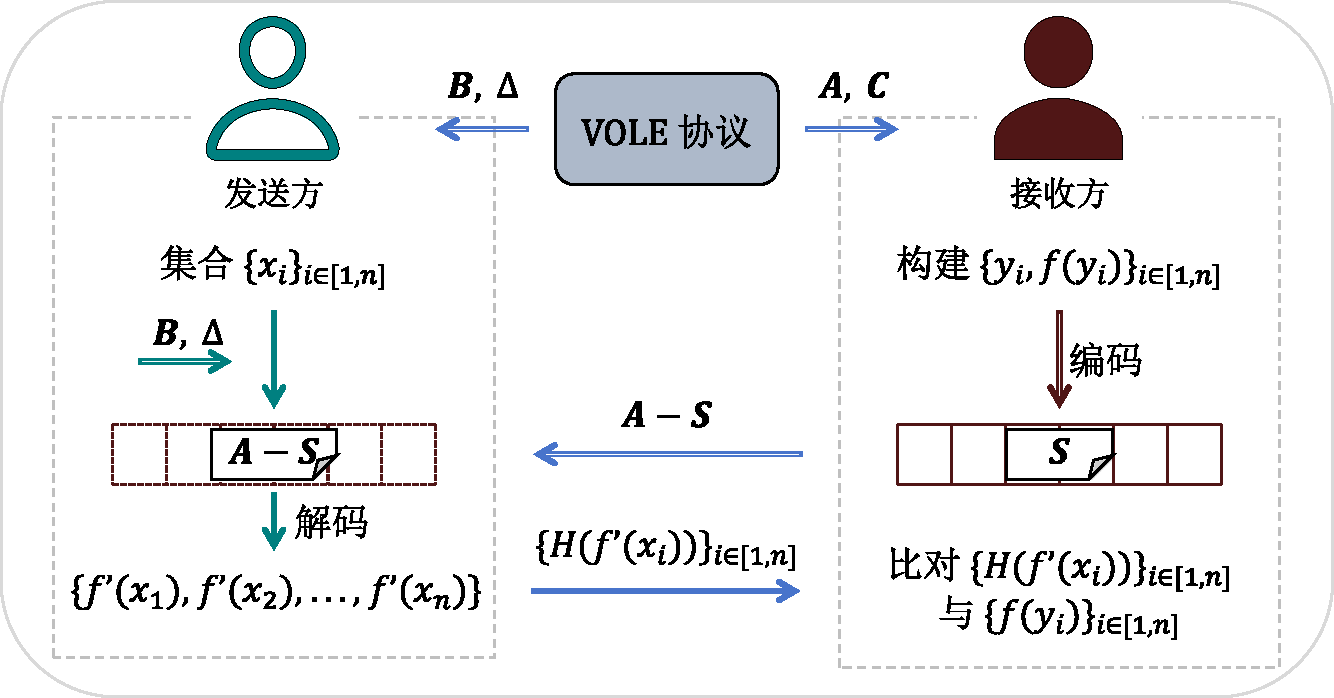
\includegraphics[width=0.9\textwidth]{figures/psi_okvs.pdf}
  \caption{VOLE-PSI 协议流程}
  \label{fig:psi_okvs}
\end{figure}
对于持有集合 $Y=\{y_i\}_{i\in [1,n]}$ 的接收方,首先将集合中的每个元素看作键,并生成对应的值 $\{f(y_i)\}_{i\in [1,n]}$,并且满足:
\begin{equation}
  f(y_i) = \mathsf{H}(\mathsf{Decode}(\mathbf{C}, y_i)),
\end{equation}
其中 $\mathsf{H}$ 为随机谕言机 (random oracle),$\mathsf{Decode}$ 为不经意键值存储中的解码算法。
然后接收方可以将键值型数据 $\{(y_i, f(y_i))\}_{i\in [1,n]}$ 编码成不经意键值存储结构 $\mathbf{S}$。
接收方将 $\mathbf{A} - \mathbf{S}$ 发送给发送方。
发送方使用 $\mathbf{B}$ 和 $\Delta$ 计算 $\mathbf{B}'$,如下所示:
% $\Delta \cdot \mathbf{S} + \mathbf{B}$,可以计算:
\begin{equation}
  \mathbf{B}' = \mathbf{B} + \Delta\cdot (\mathbf{A} - \mathbf{S}).
\end{equation}
% \begin{align}
%   \Delta \cdot \mathbf{S} + \mathbf{B} & = \Delta \cdot (\mathbf{A} - \mathbf{S}) + \mathbf{B} \\
%   & = \Delta \cdot \mathbf{A} + \mathbf{B} - \Delta \cdot \mathbf{S} \\
%   & = \mathbf{C} - \Delta \cdot \mathbf{S}.
% \end{align}
对于集合 $X=\{x_i\}_{i\in [1,n]}$ 中的每一个元素 $x_i$,发送方使用不经意键值存储的 $\mathsf{Decode}$ 算法进行解码,计算 $f'(x_i)$,如下所示:
\begin{align}
  f'(x_i) = \Delta \cdot \mathsf{Decode}(\mathbf{S}, x_i) + \mathsf{Decode}(\mathbf{B'}, x_i).
\end{align}
发送方使用与接收方相同的 $\mathsf{H}$ 得到新的集合 $\{\mathsf{H}(f'(x_i))\}_{i\in [1,n]}$,并将该集合返回给接收方。
根据 VOLE 中的线性关系以及\textbf{定义~\ref{def:okvs}}~中 $\mathsf{Decode}$ 算法的性质,当集合 $X$ 中存在与 $Y$ 有交集的元素时,即 $x_i \in Y$ 时,有:
\begin{align}
  f'(x_i) & = \Delta\cdot \mathsf{Decode}(\mathbf{S}, x_i) + \mathsf{Decode}(\mathbf{B}', x_i) \\
  & = \Delta \cdot f(x_i) + \mathsf{Decode}(\mathbf{B}, x_i) + \mathsf{Decode}(\Delta\cdot(\mathbf{A}-\mathbf{S}), x_i) \\
  & = \Delta\cdot f(x_i) + \mathsf{Decode}(\mathbf{B}, x_i) + \Delta\cdot\mathsf{Decode}(\mathbf{A}, x_i) - \Delta \cdot f(x_i) \\
  & = \mathsf{Decode}(\mathbf{B}, x_i) + \Delta \cdot \mathsf{Decode}(\mathbf{A}, x_i) \\
  & = \mathsf{Decode}(\mathbf{C}, x_i).
\end{align}
接收方只需要根据 $\mathbf{C}$ 可以直接计算 $\{\mathsf{Decode}(\mathbf{C}, y_i)\}_{i\in [1,n]}$,再与发送方返回的结果进行比对便能得到 $X\cap Y$ 的交集结果。

% 其中一个核心设计是基于向量不经意线性评估的不经意伪随机函数 (Oblivious Pseudorandom Function, OPRF),简称为 VOLE-PIR。
% 这里需要分别说明向量不经意线性评估和不经意伪随机函数的含义。
% 向量不经意线性评估通常被用于构造各种高效的安全多方计算协议,它的特点是具有较低的通信复杂度。
% 它的功能随机生成长度为 $m$ 的向量 $\mathbf{A}, \mathbf{B}, \mathbf{C}$,以及元素 $\Delta$,并且 $\mathbf{A}, \mathbf{B}, \mathbf{C}$ 满足线性关系:$\mathbf{C} = \Delta \cdot \mathbf{A} + \mathbf{B}$。
% 协议参与的接收方得到向量 $\mathbf{A}$ 和向量 $\mathbf{C}$,而发送方得到向量 $\mathbf{B}$ 和 $\Delta$。
% 不经意伪随机函数是一个两方协议,它的作用是在一方持有伪随机函数 $F_k(\cdot)$ 的密钥 $k$,另一方持有输入 $\{x_1, x_2, \dots, x_n\}$ 的情况下,让双方(或其中一方)获得伪随机函数结果,但不会获得除了结果之外的任何信息。

% 持有输入的一方获得对应的伪随机函数结果 $\{F_k(x_1), F_k(x_2), \dots, F_k(x_n)\}$,持有密钥的一方不获得任何信息。

% 基于向量不经意线性评估的不经意伪随机函数的构造建立在 VOLE 协议之上,

\subsection{SKE-PSU}

SKE-PSU~\cite{zhang2023linear}是结合不经意传输 (Oblivious Transfer,OT) 和多点反向隐私成员测试 (Multi-Query Reverse Private Membership Test, mq-RPMT) 设计的隐私集合求并方案。
其中的 mq-RPMT 构造中使用到了不经意键值存储结构。
在介绍具体方案之前,我们首先简单介绍不经意传输和多点反向隐私成员测试的含义。

不经意传输是一种常见的安全多方计算协议。
最基础的不经意传输协议是 1-out-of-2 OT,其系统模型如图~\ref{fig:ot_protocol}~所示。
\begin{figure}[ht]
  \centering
  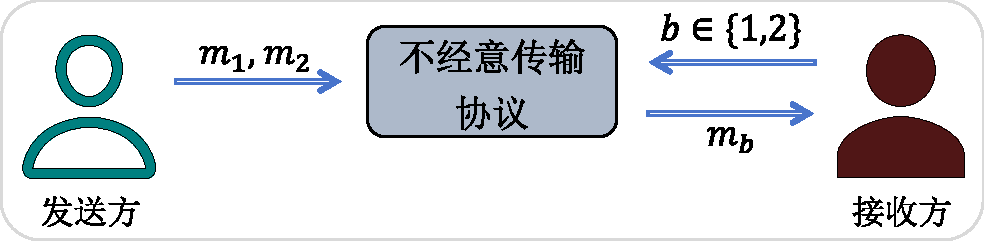
\includegraphics[width=0.72\textwidth]{figures/ot_pro.pdf}
  \caption{1-out-of-2 不经意传输系统模型}
  \label{fig:ot_protocol}
\end{figure}
其中发送方有两个消息,分别为 $m_1$ 和 $m_2$,而接收方想获取其中的一个消息 $m_b, b\in\{1,2\}$。
通过执行 1-out-of-2 OT 协议之后,接收方获得了消息 $m_b$ 但并不知道另一个消息的信息,而发送方不知道接收方想要获取的是哪个消息。
由 1-out-of-2 OT 可以扩展到 1-out-of-n OT,即接收方可以获取到发送方 $n$ 个消息中的一个,但发送方并不能判断接收方获取的具体是哪个消息。

多点反向隐私成员测试是一个两方协议,它的作用是判断发送方提供的元素 $x_i$ 是否属于接收方的集合 $Y$,并让接收方获得判断结果,而发送方不获得任何信息。
在执行该协议之后,接收方便能知道哪些序号的元素是不在集合 $Y$ 中的,之后就可以通过不经意传输协议获取这些元素,得到并集结果。
% 之后便能通过
早期的反向隐私成员测试协议~\cite{kolesnikov2019scalable}一次只能判断一个元素,也被称为单点反向隐私成员测试。
SKE-PSU~\cite{zhang2023linear}中借助不经意键值存储结构和 VODE (Vector Oblivious Decryption-then-Matching) 协议实现了多点反向隐私成员测试协议,也就是可以一次判断多个元素。
这里的 VODE 也是一种作用于两方的协议,假设 $\mathcal{E} = (\mathsf{Setup}, \mathsf{KeyGen}, \mathsf{Enc}, \mathsf{Dec})$ 为一个抗选择明文攻击安全的对称加密机制,VODE 的功能描述如下:
\begin{itemize}
  \item 接收方持有明文 $s$ 以及由 $\mathsf{KeyGen}$ 生成的密钥 $k$。
  \item 发送方持有集合 $\{s_1^*, s_2^*, \dots, s_n^*\}$,其中每个元素都来自 $\mathcal{E}$ 的密文空间。
  \item 对于 $i\in [1,n]$,计算 $s_i' = \mathsf{Dec}(k, s_i^*)$。如果 $s_i' = s$,令 $b_i = 1$,否则 $b_i = 0$。
  \item 接收方得到判断结果 $\{b_i\}_{i\in [1,n]}$。
\end{itemize}
% 关于 VODE 的构造
在有了 VODE 协议的基础上,我们可以构建多点反向隐私成员测试,其流程如图~\ref{fig:psu_okvs}~所示。
\begin{figure}[ht]
  \centering
  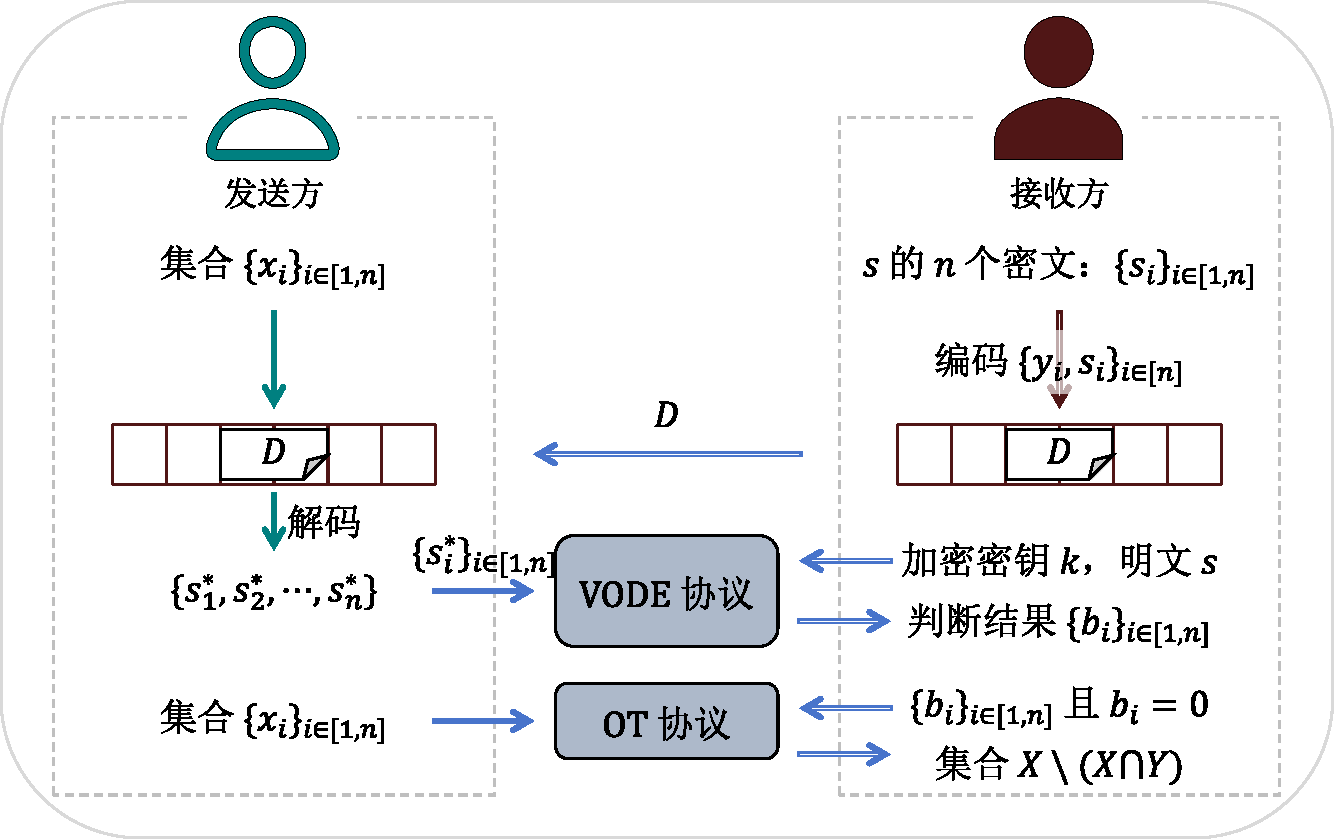
\includegraphics[width=0.9\textwidth]{figures/psu_okvs.pdf}
  \caption{SKE-PSU 协议流程}
  \label{fig:psu_okvs}
\end{figure}
我们依然假设发送方持有集合 $X = \{x_i\}_{i\in [1,n]}$,接收方持有集合 $Y = \{y_i\}_{i\in [1,n]}$,协议流程描述如下:
\begin{itemize}
  \item 接收方随机生成标识字符串 $s$,使用 $\mathsf{KeyGen}$ 生成密钥 $k$,并使用加密机制 $\mathcal{E}$ 将 $s$ 加密 $n$ 次,得到 $\{s_1, s_2, \dots, s_n\}$。
  \item 接收方构造键值型数据 $\{(y_1, s_1), (y_2, s_2), \dots, (y_n, s_n)\}$,并使用不经意键值存储的 $\mathsf{Encode}$ 编码成 $D$,将 $D$ 发送给发送方。
  \item 发送方收到 $D$ 之后,便可以用自己的集合 $X$ 作为输入,使用不经意键值存储的 $\mathsf{Dncode}$ 算法解码成 $\{s_1^*, s_2^*, \dots, s_n^*\}$。
  \item 接收方和发送方执行 VODE 协议,发送方输入 $\{s_1^*, s_2^*, \dots, s_n^*\}$,接收方输入 $(k, s)$。因为 VODE 的作用是判断密文 $s_i^*$ 与明文 $s$ 能否匹配,所以最终接收方获取到一系列判断结果 $\{b_1, b_2, \dots, b_n\}$。
  \item 在得到判断结果的输出后,接收方便能通过不经意传输协议,从发送方获取到不属于集合 $Y$ 中的元素,最终得到 $X\cup Y$ 的结果。
\end{itemize}
得益于不经意键值存储的性质,当 $x_i \in Y$ 时,发送方计算出的 $s_i^*$ 就是 $s$ 的密文。
而不经意的性质确保发送方无法知道 $x_i$ 是否属于 $Y$,避免发送方获取到额外的信息。
而当计算出判断结果 $\{b_i\}_{i\in[1,n]}$之后,接收方也只知道当 $b_i=1$ 时,对应集合 $X$ 中序号为 $i$ 的元素存在于集合 $Y$ 中,但并不能知道 $x_i$ 的具体信息,从而防止接收方获得交集信息。

% SKE-PSU~\cite{zhang2023linear}中的多查询反向隐私成员测试使用了向量不经意
% 相比隐私集合求交协议,隐私集合求并要求的是接收方只能获取到并集信息,而不能获取到交集内容。
% 因此就需要
% 隐私计算
% 反向隐私成员测试 (Reverse Private Membership Test, RPMT)
% SKE-PSU~\cite{zhang2023linear}

\section{总结}

这一节我们主要介绍了布隆过滤器及其衍生的数据结构在对称可搜索加密、隐私信息检索和隐私集合运算上的应用。
这些数据结构之所以能够广泛应用在各种不同的隐私保护协议之中,主要有以下几个方面的原因:
\begin{itemize}
  \item 较低的空间开销:在设计隐私保护计算协议尤其涉及到双方交互的协议时,影响性能的因素之一便是通信开销。
  而过滤器或者不经意的键值存储本身就是一种压缩率非常高的结构,引入这些结构会大大降低协议的通信开销。比如在隐私集合运算过程中,交互双方并不会直接发送(加密后的)集合信息,而是采取将集合表示为过滤器或不经意键值存储结构后再发送。
  \item 灵活的编码形式:布隆过滤器能够将集合中的元素编码成 $0/1$ 比特串的形式,从而可以直接应用到输入为比特向量的加密机制中(比如 HXT 中的 SHVE);异或型过滤器和不经意键值存储能够将键值型数据重新编码。
  % 成全新的向量形式,
  % 进数据结构,
  因此只要是任意键值型数据(比如 XorMM 中的索引,ChalametPIR 中的数据条目结构),都可以直接编码成向量的数据结构形式。
  \item 成员测试的能力:过滤器设计的初衷就是实现成员测试。
  正因为其拥有成员测试的能力,因此可以用于查询协议中做条件判断。
  比如在 HXT 中判断多个搜索关键词是否与文件标识匹配,ChalametPIR 中判断那些数据符合用户的请求。
  而对于异或型过滤器和不经意键值存储来说,它们还具有不经意的性质,也就是对任意输入都可以生成一个输出。
  比如在 XorMM 协议中服务器对 $\ell$ 个查询需要返回 $\ell$ 个输出,在 VOLE-PSI 协议中,发送方对集合中每个元素 $x_i$,都有对应的输出 $f'(x_i)$,在 SKE-PSU 协议中,发送方对集合中每个元素 $x_i$,都有对应的输出 $s_i^*$。这样不经意性保证让一方不获取任何消息的同时,为另一方提供成员测试的功能。
  % 实现更加安全的方案(比如 HXT 隐藏 KPRP)
\end{itemize}


% 本文的前两章主要介绍了布隆过滤器及其衍生的新型数据结构的构造和性能,希望能让大家对这些数据结构有一个初步认识。
% 最后一章结合三个常见的隐私保护协议介绍了这些数据结构是如何应用的,希望能让大家了解到现有的一些设计方法,为设计隐私保护协议提供新思路。

这一节的主要目的是希望通过介绍这些数据结构在隐私保护协议上的应用,让大家了解到现有的一些通用方法,为设计隐私保护协议提供新的思路。
% 目前这些数据结构的应用
从我们列出的相关工作也可以看出,布隆过滤器和布谷鸟过滤器在隐私保护协议中已经应用得很成熟,而异或型过滤器和不经意键值存储的应用近几年才刚刚开始。
我们可以多关注后两种数据存储结构,或许能为我们构建方案提供更好的帮助。
% 尝试在不同隐私保护协议中

% 本文的目的是希望能够通过对这些数据结构进行总结,让大家对过滤器及其相关新型数据的构造、性能以及如何使用有一个初步的认识,为设计隐私保护相关协议提供新思路。
% 有了理论上的了解只是一个开始,我们应该知道如何去应用。
% 希望通过本文在最后列举的几个例子能够给各位
% 本文介绍的这些新型数据结构还具有

% 具有较低的空间开销、
% 编码能力
% 判断能力
% 线性可加能力
